\section{Gear}
\index{Gear}

Unlike other systems that track individual items, inventory weight, and resource management, \wyrd keeps gear streamlined and abstract. Instead of worrying about encumbrance, ammunition, or minor supplies, characters only track \textbf{gear that truly matters}. This means that most mundane equipment is assumed to be available when reasonable, and only items that provide a mechanical or narrative advantage are recorded.

\subsection{Gear as Traits}
Gear in \emph{The Wyrd Engine} functions similarly to Traits. Instead of listing specific damage values or weight, an item has a \textbf{trait} that defines its benefit in play. 

\wyrd gear should:
\begin{itemize}
    \item Provide a \emph{specific mechanical advantage} (e.g. \textbf{+2 bonus} to a relevant skill check).
    \item Offer a \emph{unique function} that enables new actions.
    \item Be \emph{narratively significant}—not just generic supplies.
\end{itemize}

Notice that the first two requirements closely resemble the description of traits. This is intentional, as it allows gear to have game mechanic effects while reusing the same rules already introduced.

\begin{CommentBox}{Example Gear}
	\textbf{Detective’s Magnifying Glass}  
	\emph{Gain +2 to Investigate when examining tiny details or analysing documents.}

	\textbf{Clockwork Grappling Hook}  
	\emph{Once per session, escape or reach a high place instantly.}

	\textbf{Masterwork Dueling Pistol}  
	\emph{Gain +2 to Shoot in one-on-one confrontations.}

	\textbf{Encrypted Notebook}  
	\emph{Allows the player to store complex cyphers or hidden information that only they can decode.}

	\textbf{Hidden Blade}  
	\emph{Use \textbf{Stealth} instead of \textbf{Fight} in a surprise attack.}

	\textbf{Reinforced Trench Coat}  
	\emph{Gain +2 to \textbf{Physique} when resisting blunt force trauma.}
\end{CommentBox}

\subsection{Using Gear in Play}
Gear should not be micromanaged but used to define a character’s tools, specialities, and advantages. If an item logically fits a character’s concept—such as a detective having a notebook or a thief carrying lockpicks—it’s assumed to be available without taking up a slot. Only equipment that \emph{enhances gameplay} or \emph{creates narrative opportunities} should be explicitly listed.

The trait-like behaviour of gear can also serve a second purpose in \emph{The Wyrd Engine}: Gear provides a way to boost characters abilities---quite substantially---by \textbf{+2} bonuses whenever the gear's requirements are met. For advancing characters when preparing them for a battle with the final boss of a scenario, a Game Master can gift the players with increasingly powerful gear as rewards for minor battles. Using gear is a simple way to handle character advancement in \emph{The Wyrd Engine}.

Once player characters start relying on such powerful items, a Game Master has a second trick to add excitement: unlike traits, gear can be taken away again. Recovering stolen gear necessary for the final confrontation is an excellent way to add side-quests to a game session.

\vspace*{\fill}

\begin{GmTips}
	If a player asks, “Do I have this item?” consider whether it fits their role and background. If it makes sense, they do. If it would provide a major advantage, it should be a tracked piece of gear with a trait.
\end{GmTips}

\vspace*{\fill}
\begin{center}
    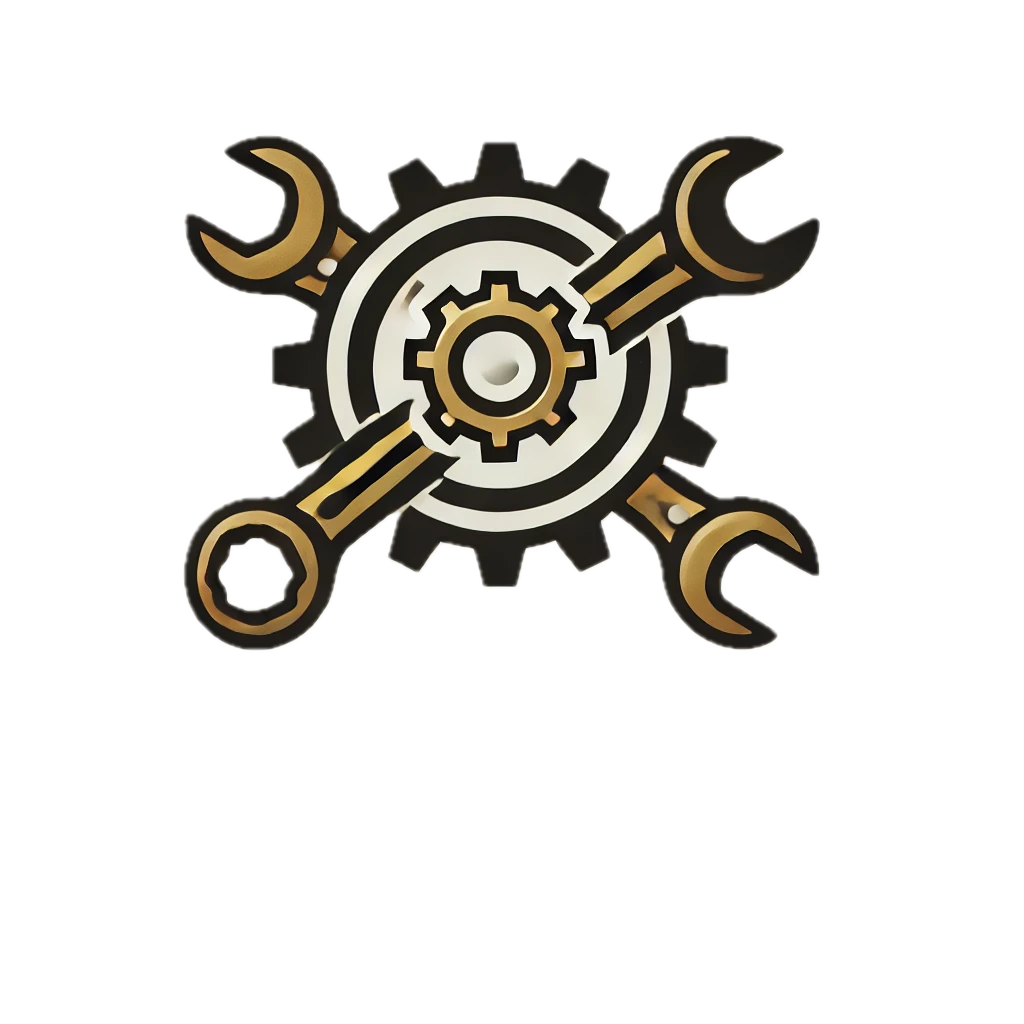
\includegraphics[width=\linewidth]{img/separt/gear-logo}
\end{center}
\vspace*{\fill}

% Switching column with slightly nicer balancing
\end{multicols}
\begin{multicols}{2}